\documentclass[english]{article}
\usepackage[italian]{babel} 
\usepackage[T1]{fontenc}
\usepackage[utf8x]{inputenc}
\usepackage{float}
\usepackage{graphicx}
\usepackage{placeins}
\usepackage{wrapfig}
\includeonly{                 
./Cap1/1,
./Cap2/2,
./Cap3/3,
./Cap4/4,
./Cap5/5,
./Appendici/A
}


\makeatletter
\usepackage[a4paper,top=2cm,bottom=2cm,left=2cm,right=2cm]{geometry}
\usepackage{enumitem}
\usepackage{subfig}
\usepackage{sidecap}
\usepackage{newclude}
\usepackage{amsmath}
\usepackage{amssymb}
\usepackage{epstopdf}
\usepackage{fancyhdr}
\usepackage{booktabs,array}
\usepackage[output-decimal-marker={,}]{siunitx}
\usepackage{color}
\usepackage{empheq}
\usepackage{graphicx}
\usepackage{hyperref}
\usepackage{hf-tikz}
\usepackage{tikz}
\usepackage{bodegraph}
\usepackage{schemabloc}
\usetikzlibrary{circuits}
\usepackage{tabularx}
\usepackage{pgfplots}
\usepackage[siunitx]{circuitikz}
\usetikzlibrary{decorations.pathreplacing}


% SCHEMA A BLOCCHI %
\newcommand{\trippleSpacing}{\phantom{aaa}}	% spazio di tre caratteri
\newcommand{\singleSpacing}{\phantom{a}}	% spazio di un carattere
		
\tikzstyle{block} = [draw, rectangle, minimum height=3em, minimum width=2em]
\tikzstyle{sum} = [circle, minimum width=12pt, draw, inner sep=0pt, path picture={\draw (path picture bounding box.south east) -- (path picture bounding box.north west) (path picture bounding box.south west) -- (path picture bounding box.north east);}]
\tikzstyle{input} = [coordinate]
\tikzstyle{output} = [coordinate]
\tikzstyle{pinstyle} = [pin edge={to-,thin,black}]

\tikzstyle{my right of} = [right of=#1.east]



\hyphenation{italian}
\lhead{Laboratorio di Controlli}
\rhead{Esperienza 1}

\makeatother

\usepackage{babel}

\begin{document}



\begin{titlepage} 

\begin{center}
\begin{Large} \textbf{UNIVERSITA' DEGLI STUDI DI PADOVA} \\
 \end{Large} \vspace{1cm}
 \begin{Large} \textbf{Corso di Laurea Magistrale in Ingegneria dell'Automazione}\\
 \end{Large} \vspace{2cm}
\begin{Large} Corso di Laboratorio di Controlli \end{Large}
\par\end{center}

\begin{center}
\begin{Large}Esperienza 2: Progettazione di controllori PID e con retroazione stato per un motore elettrico\\
 \end{Large}
\par\end{center}

\begin{center}
\vspace{2cm}
\begin{figure}[!htb]
\centering 
\includegraphics[width=8cm]{./figure/unipd}\\
 
\end{figure}

\par\end{center}

\begin{center}
 \vspace{2cm}
 \begin{Large} Dal Lago Nicola - 1104228 \\
 \end{Large} \vspace{2cm}
 \begin{Large} Anno Accademico 2014-2015 \end{Large} 
\par\end{center}

\end{titlepage}

\tableofcontents


\newpage
\include*{./Cap1/1}
\include*{./Cap2/2}
\section{Modellizzazione}
\label{sec:Modelizzazione}
	
	Nel corso di questa esperienza, viene impiegato un motore elettrico a corrente continua. Il motore è controllato tramite un segnale in tensione e fornisce in output l'attuale posizione del carico, attraverso l'utilizzo di un encoder.
	
	\subsection{Modellizzazione del motore}
	\label{subsec:ModellizzazioneMotore}
	
		Un motore elettrico in corrente continua, può essere suddiviso in due parti, statore e rotore. \newline
		Lo statore ha il compito di indurre un campo magnetico $B$, attraverso l'uso di materiali ferromagnetici e correnti elettriche. \newline
		Il rotore è composto da un elevato numero di spire percorse da corrente $i$ e immerse nel campo magnetico prodotto dallo statore. \newline
		Come è noto dalla \textit{legge di Faraday}, una spira in tale situazione produce una forza elettro motrice $f.e.m.$, pari all'opposto della derivata rispetto al tempo del flusso concatenato dalla spira
	
		\begin{equation}
			f.e.m. = -\frac{d\theta(t)}{dt} = AB\sin(\alpha(t))\cdot\frac{d\alpha(t)}{dt}
			\label{eq:fem}
		\end{equation}
	
		\noindent dove $A$ è l'area della spira, e $\alpha$ è l'angolo tra il vettore campo magnetico e il versore perpendicolare alla spira con verso dato dalla regola della vite destrorsa. \newline
		Si può quindi ricavare anche il momento torcente totale $\tau_{TOT}$ di ciascuna spira come
	
		\begin{equation}
			\tau_{TOT} = ABi\sin{\alpha(t)}
			\label{eq:momentoTorcente}
		\end{equation} 
	
		\noindent Riassumendo, possiamo scrivere la \textbf{dinamica elettro-meccanica} del rotore:
		
		\begin{equation}
			\begin{cases}
				f.e.m. = -AB\omega = -k_{\phi}\omega \\
				\tau_{TOT} = ABi = k_{\phi}i
			\end{cases}
			\label{eq:dinamecaElettroMeccanica}
		\end{equation}
	
		\noindent dove, con $\omega$ si indica la velocità angolare del rotore e con $k_{\phi}$ la \textit{costante elettrica} fornita da datasheet.\newline
		Per la \textbf{dinamica meccanica}, supponendo di avere un attrito viscoso descritto come $\tau_{attr} = -b\omega$, possiamo ricavarne l'equazione utilizzando il momento di inerzia $J$:
	
		\begin{equation}
			J\frac{d\omega}{dt} = k_{\phi}i - b\omega
			\label{eq:uscita}
		\end{equation}  
	
		\noindent si noti come questa equazione può essere interpretata come l'uscita del nostro sistema motore, in quanto è una equazione differenziale in funzione della velocità angolare del motore. \newline
		Passando alla \textbf{dinamica elettrica}, possiamo pensare il motore come una serie di una resistenza $R$, un generatore di forza elettromotrice $f.e.m.$ e una induttanza $L$; ai capi di tale serie, viene applicata una tensione $v_m$, il nostro controllo. Possiamo quindi scrivere l'equazione di controllo
	
		\begin{equation}
			v_m -k_{\phi}\omega = Ri + L \frac{di}{dt}
			\label{eq:controllo}
		\end{equation}    
	
		\noindent Ora possiamo unire le equazioni di uscita e di controllo, e interpretare $i$ e $\omega$ come le variabili di stato
	
		\begin{equation}
			\begin{cases}
				v_m = Ri + L\frac{di}{dt} + k_{\phi}\omega \\
				J\frac{d\omega}{dt} = -b\omega + k_{\phi}i
			\end{cases}
			\label{eq:dinamicaComplessiva}
		\end{equation}
	
		\noindent e applicando la \textit{trasformata di Laplace} scriviamo
	
		\begin{equation}
			\begin{cases}
				V_m(s) = RI(s) +sLI(s) + k_{\phi}\Omega(s)\\
				Js\Omega(s) = -b\Omega(s) + k_{phi}I(s)	
			\end{cases}
			\label{eq:dinamecaComplessivaLaplace}
		\end{equation}
	
		\noindent Con dei semplici passaggi algebrici è possibile ottenere
	
		\begin{equation}
			\Omega(s) = P(s)V_m(s) = \frac{k_{\phi}}{(R+sL)(b+SJ)+k_{\phi}}\cdot V_m(s)
			\label{eq:funzioneTrasferimento}
		\end{equation}
	
		\noindent dove con $P(s)$ indichiamo la funzione di trasferimento del processo. Nel caso del nostro motore, possiamo trascurare l'effetto induttivo, in quanto è di molto inferiore rispetto a tutti gli altri paramenti; ci risulta quindi una equazione di trasferimento
	
		\begin{equation}
			P(s) = \frac{k_{\phi}}{RJs + Rb +K_{\phi}^2}
			\label{eq:funzioneTrasferimentoSemplificata}
		\end{equation}
	
		\noindent Come accennato all'inizio del paragrafo, il motore è disposto di un encoder in grado di misurare solo la posizione angolare $\theta_m$ del motore, e non la velocità angolare; è possibile però ricondursi ad una funzione di trasferimento che abbia la posizione e non la velocità come parametro di uscita ricordando la relazione che le lega: 
	
		\begin{equation*}
			\frac{d\theta_m}{dt} = \omega
			\label{eq:posizioneVelocità}
		\end{equation*}
	
		\noindent e utilizzando la \textit{trasformata di Laplace} $s\Theta_m(s)=\Omega(s)$. Viene quindi aggiunto un polo in zero al processo:
	
		\begin{equation}
			P_{\theta}(s) = \frac{k_{\phi}}{s(RJs + Rb + k_{\phi}^2)}
			\label{eq:funzioneTrasferimentoMotoriduttore}
		\end{equation}
	
		\noindent Per comandare il motore in gradi rispetto alla tensione, bisogna introdurre due costanti moltiplicative che sono in grado di trasformare un valore in gradi a uno in tensione e viceversa:
	
		\begin{itemize}
			\item $K_{g2v}$ : costante moltiplicativa per passare da gradi a tensione;
			\item $K_{v2g}$ : costante moltiplicativa per passare da tensione a gradi.
			\label{item:costantiK} 
		\end{itemize}
	

	\subsection{Modellizzazione del motoriduttore}
	\label{subsec:ModellizzazioneMotoriduttore}
	
		Tipicamente un motore non viene usato direttamente per comandare un carico, ma si utilizzano una coppia di ingranaggi necessari per adattare le prestazioni del motore alle specifiche di progetto; questo tipo di configurazione viene chiamata \textit{motoriduzione}. E' necessario quindi definire nuove variabili:
	
		\begin{itemize}
			\item $N_m$ : numero denti dell'ingranaggio collegato al motore;
			\item $N_l$ : numero denti dell'ingranaggio collegato al carico;
			\item $\tau_m$ : momento torcente applicato al motore dall'ingranaggio;
			\item $\tau_l$ : momento torcente applicato al carico;
			\item $b_m$ : costante di attrito viscoso nel rotore lato motore;
			\item $b_l$ : costante di attrito viscoso nel rotore lato carico;
			\item $N = \frac{N_l}{N_m}$ : rapporto di motoriduzione.
		\end{itemize}  
	
		\noindent Inoltre il motore ha una serie di non idealità le quali ne complicherebbero di molto lo studio; riportiamo qui le semplificazioni fatte
	
		\begin{itemize}
			\item $L = 0$ : induttanza trascurabile;
			\item non c'è slittamento tra le ruote, il che implica;
			\begin{equation}
				\theta_mN_m = \theta_lN_l \Longrightarrow N_m\frac{d\theta_m}{dt}=N_l\frac{t\theta_l}{dt}
				\label{eq:nonIdealità1}
			\end{equation}
			\item non c'è dissipazione al punto di contatto, cioè le potenze rimangono costanti.
			\begin{equation}
				\tau_m\omega_m=\tau_l\omega_l \Longrightarrow \tau_m\frac{d\theta_m}{dt}=\tau_l\frac{d\theta_l}{dt}
				\label{eq:nonIdealità2}  
			\end{equation}
		\end{itemize}
	
		\noindent dall'equazione \ref{eq:nonIdealità1} e \ref{eq:nonIdealità2} otteniamo
	
		\begin{gather}
			\frac{\omega_m}{\omega_l}=\frac{N_l}{N_m}=N \Longleftrightarrow \omega_m=N\omega_l \\
			\tau_mN\omega_l=\tau_l\omega_l \Longleftrightarrow \tau_l=N\tau_m
		\label{gat:comp}
		\end{gather}
	
	
		\noindent e unendo tutto insieme nell'equazione del motore ricaviamo
	
		\begin{gather}
			\bigl(J_mN^2+J_l\bigl)\frac{d\omega_l}{dt}=-\bigl(b_mN^2+b_l\bigl)\omega_l+Nk_{\phi}i \\
			J_{eq}\frac{d\omega_l}{dt}=-b_{eq}\omega_l+k_{\phi,eq}i
			\label{gat:motoriduttore}
		\end{gather}
	
		\noindent Si può vedere come la forma delle equazioni del motore e del motoriduttore siano praticamente uguali, ciò che cambia è il valore delle costanti. 
		\noindent I dati di targa del motore presente in laboratorio sono riassunti nella tabella \ref{tab:parametri}. 
		
		\begin{table}[H]
			\centering
			\begin{tabular}{ccc}
				\toprule
				\textbf{Parametro} & \textbf{Valore} & \textbf{Unità di misura}\\
				\midrule
				$K_{g2v}$ & \SI{0,0284}  & $Volt/rad$       \\
				$K_{r2v}$ & \SI{1,63}    & $Volt/rad$       \\
				$N$       & \SI{14}      &                  \\
				$k_\phi$  & \SI{0,00767} & $Volt/(rad/sec)$ \\
				$J_m$     & \SI{3,87e-7} & $kg\cdot m^2$    \\ 	
				$J_l$     & \SI{3,42e-5} & $kg\cdot m^2$    \\
				$R$       & \SI{2,6}     & $\Omega$         \\
				$L$       & \SI{0,18e-3} & $H$              \\
				\bottomrule
			\end{tabular}
			\caption{Dati di targa del motore}
			\label{tab:parametri}
		\end{table}
	
		\noindent $b_m$ e $b_l$ non sono noti a priori, ma per il nostro laboratorio vengono considerati nulli, come $L$. \newline
		Come prima, anche in questo caso l'encoder ci fornisce la posizione angolare del carico e non la sua velocità, ma applicando gli stessi ragionamenti si può arrivare a formulare l'equazione finale del processo:	
		
		\begin{equation}
			P_{\theta}(s) = 
			%\tikzmarkin{right delim frac}(0.6,2.8)(-0.1,0.6)
			\frac{Nk_{\phi}}{s\bigl( R(J_mN^2+J_l) \bigl) + N^2k_{\phi}^2}
			%\tikzmarkend{right delim frac}
			\label{eq:FunzioneTrasferimentoComplessiva}
		\end{equation}
		
		\noindent mentre la vera funzione di trasferimento ``osservata'' dal motore è moltiplicata per il fattore $K_{r2v}$, risulta allora
		
		\begin{equation*}
			P_{\theta}'(s)= K_{r2v}\cdot P_{\theta}(s) \approx \frac{375}{s(s+40)}
		\end{equation*}
		
		\begin{figure}[H]
			\centering
			\subfloat[][\emph{Diagramma di Bode del modulo.}]{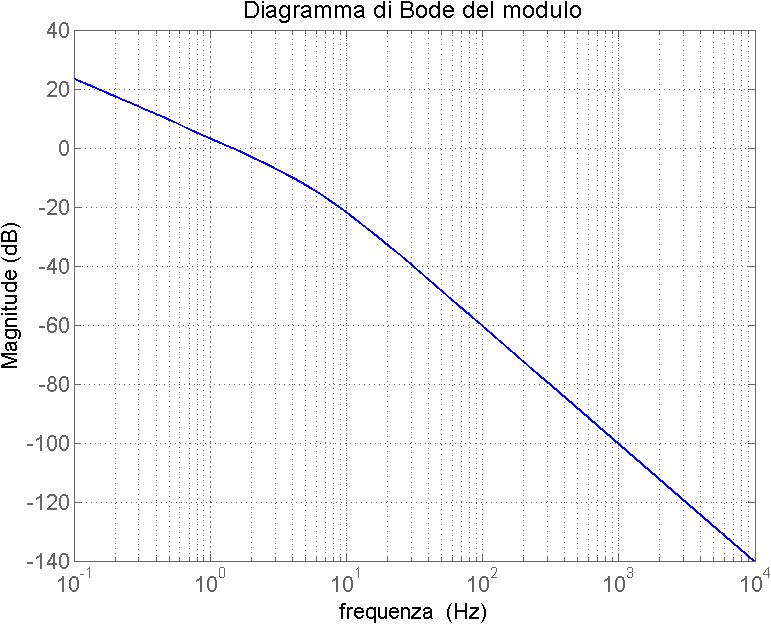
\includegraphics[width=.48\textwidth]{./figure/bode_mag.png}}\label{subfig:diagrammaBode} \quad
			\subfloat[][\emph{Diagramma di Bode della fase.}]{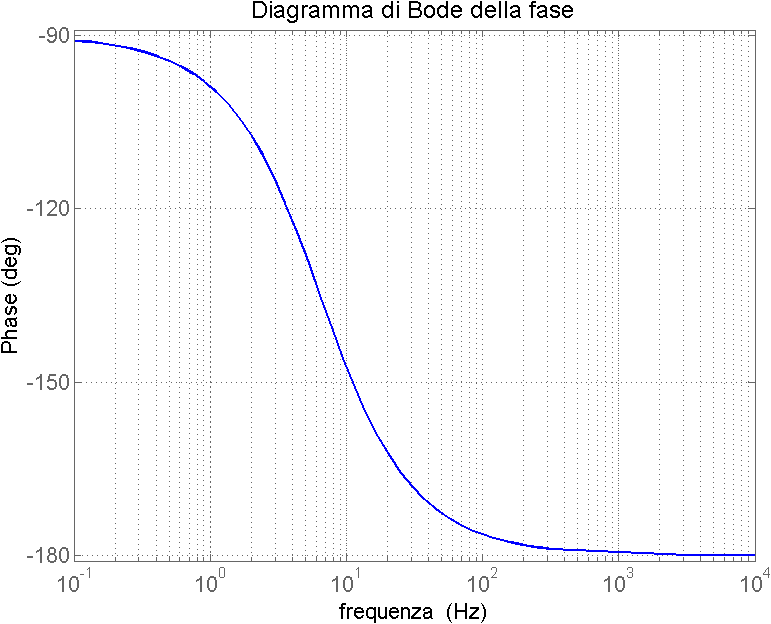
\includegraphics[width=.48\textwidth]{./figure/bode_phase.png}}\label{subfig:mappaZeriPoli}
			\caption{Diagramma di Bode di modulo e fase del processo relativo al motore.}
			\label{fig:diagrammiMotore}
		\end{figure}	
		
		\noindent In figura \ref{fig:diagrammiMotore} è rappresentato l'andamento di modulo e fase della funzione di trasferimento $P_{\theta}'(s)$.
		
	\subsection{Modellizzazione in spazio di stato}
	\label{subsec:ModelloStato}
	
	Una delle possibili rappresentazioni di un processo, insieme a quella in funzione di trasferimento usata fin'ora, è quella in spazio di stato. E' possibile scrivere il sistema come una coppia di equazioni lineari descritte come
		
	\begin{equation}
		\begin{cases}
			\dot{x}(t)=Ax(t)+Bu(t) \\
			y(t)=Cx(t)+Du(t)
		\end{cases}
	\end{equation}	
		
	\noindent dove $x(t)$ è lo stato, $u(t)$ l'ingresso e $y(t)$ l'uscita. Si dimostra che il processo in funzione di trasferimento può essere scritto come $P(s)=C(sI-A)^{-1}B+D$, ma quello che tipicamente si fa, è di ricavare direttamente le il modello dalle equazioni fisiche. Si procederà anche qui in questo modo. Le equazioni fisiche del motore, ricavate nella sessione \ref{sec:Modelizzazione}, sono divise in quattro parti:
		
	\begin{itemize}
		\item elettrica: $V_m(t)=Ri(t)+k_{\phi}^{eq}\dot{\Theta}_l$
		\item elettromeccanica: $\tau_l(t)=k_{\phi}^{eq}i(t)$
		\item meccanica: $J_{eq}\ddot{\Theta}_l=-b_{eq}\dot{\Theta}_l+\tau_l(t)$
		\item sensore: $V_{out}(t)=K_T\Theta_l$
	\end{itemize}  
		
	\noindent Come stato si è preso l'angolo del carico e la sue velocità angolare, $x=[\Theta_l \singleSpacing \dot{\Theta}_l]^T$, come ingresso $u=V_m$ e come uscita $y=V_{out}$. Si può riscrivere le prime tre equazioni nel seguente modo
		
	\begin{gather}
		i(t)=\frac{V_m(t)-k_{\phi}^{eq}\dot{\Theta}_l(t)}{R} \\
		\tau_l(t)=k_{\phi}^{eq}\Bigl(\frac{1}{R}V_m(t)-\frac{k_{\phi}^{eq}}{R}\dot{\Theta}_l\Bigl) \\
		J_{eq}\ddot{\Theta}_l=-b_{eq}\dot{\Theta}_l+\frac{k_{\phi}^{eq}}{R}V_m(t)-\frac{(k_{\phi}^{eq})^2}{R}\dot{\Theta}_l=-\Bigl(b_{eq}+\frac{(k_{\phi}^{eq})^2}{R}\Bigl)\dot{\Theta}_l(t)+\frac{k_{\phi}^{eq}}{R}V_m(t)
	\end{gather}  
		
	\noindent e allora
		
	\begin{equation}
		\begin{cases}
			\ddot{\Theta}_l(t)=-\Bigl(\frac{b_{eq}}{J_{eq}}+\frac{(k_{\phi}^{eq})^2}{R}\Bigl)\dot{\Theta}_l(t)+\frac{k_{\phi}^{eq}}{R}V_m(t) \\
			V_{out}(t)=K_T\Theta_l
		\end{cases}
	\end{equation}
		
	\noindent e riscrivendo il tutto in forma di stato esplicitando le matrici $A$, $B$, $C$ e $D$, si ottiene
		
	\begin{equation}
		\begin{cases}
			\begin{bmatrix}
				\dot{\Theta}_l(t)  \\
				\ddot{\Theta}_l(t) \\
			\end{bmatrix}
			=
			\begin{bmatrix}
				0 & 1                                  \\
				0 & -\frac{b_{eq}}{J_{eq}}-\frac{(k_{\phi}^{eq})^2}{R} \\
			\end{bmatrix}
			\begin{bmatrix}
				\Theta_l(t)       \\
				\dot{\Theta}_l(t) \\
			\end{bmatrix}	
			+
			\begin{bmatrix}
				0                       \\
				\frac{k_{\phi}^{eq}}{R} \\
			\end{bmatrix}
			V_m(t) \\
			V_{out}(t)=
			\begin{bmatrix}
				k_T & 0 \\
			\end{bmatrix}
			\begin{bmatrix}
				\Theta_l(t)       \\
				\dot{\Theta}_l(t) \\
			\end{bmatrix}
			+
			\begin{bmatrix}
				0 \\
			\end{bmatrix}
			V_m(t)											
		\end{cases}
	\end{equation}
		
	\noindent Essendo questo un sistema \textit{SISO}, la matrice di raggiungibilità ha rango pieno se e solo se il suo determinante è pari a zero. In questo caso
		
	\begin{equation}
		\mathcal{R}=[A|AB]=
		\begin{bmatrix}
			0 & \frac{k_{\phi}^{eq}}{RJ_{eq}} \\
			\frac{k_{\phi}^{eq}}{RJ_{eq}} & \star \\
		\end{bmatrix}
	\end{equation}
		
	\noindent ha rango 2, il che implica che il sistema considerato è raggiungibile. Lo stesso valo per la matrice di osservabilità
		
	\begin{equation}
		\mathcal{O}=
		\left[
		\begin{array}{cc}
			C  \\ \hline
			CA \\
		\end{array}
		\right]
		=
		\begin{bmatrix}
			k_T & 0   \\
			0   & k_T \\
		\end{bmatrix}
	\end{equation} 
		
	\noindent che ha rango pieno, il  che implica un sistema osservabile. La raggiungibilità ci garantisce che per ogni condizione iniziale, posso portare il sistema in qualunque stato. Mentre l'osservabilità ci permette di ricavare lo stato conoscendo gli ingressi e le uscite.
\include*{./Cap4/4}
\include*{./Cap5/5}
	

\appendix	
		
\section{Progettazione in frequenza per un sistema del secondo ordine}
	\label{app:sistemaSecondoordine}
	
	Una funzione di trasferimento del secondo ordine, può essere scritta in maniera del tutto generale come
	
	\begin{equation}
		H(s)=\frac{\omega_n^2}{s^2 + 2\xi \omega_ns + \omega_n^2}
		\label{eq:secondoOrdine}
	\end{equation}
	
	\noindent dove il parametro $\xi$ è il \textit{coefficiente si smorzamento} e $\omega_n$ è la \textit{pulsazione naturale non smorzata}. I poli di tale funzione di trasferimento sono una coppia complessa coniugata e si trovano ad una distanza dall'origine pari a $\omega_n$ e a un angolo $\theta=\arcsin\xi$. Una specifica naturale per le prestazione del sistema in termini di risposta in frequenza è la \textit{larghezza di banda}, definita come la frequenza massima alla quale il  sistema segue un ingresso sinusoidale in modo soddisfacente. Altro parametro importante è il valore massimo del modulo della  risposta in frequenza, denominato come picco di risonanza $S$. La larghezza di banda è una misura della prontezza di risposta e come tale corrisponde ad altri parametri, quali il tempo di salita e il tempo al picco nel dominio del tempo.
	
	\begin{figure}[H]
		\centering
		\begin{tikzpicture}[xscale=10/3]
			\begin{scope}[yscale=4/110]
				\tikzset{
					semilog lines/.style={thin, red},
					semilog lines 2/.style={semilog lines,red!50 },
					semilog half lines/.style={semilog lines 2,dotted},
					semilog label x/.style={semilog lines,
					below,font=\tiny, black},
					semilog label y/.style={semilog lines,right,font=\tiny, black}
					}
				%\UnitedB
				\semilog{0}{3}{-70}{40}
				\BodeGraph[blue]{0:3}{\POAmp{9.375}{0.025}+\IntAmp{1}}
					
				\node [below=6pt] at (1.5,-65) {$\omega$ \singleSpacing (rad/s)};
				\node [rotate=90] at (-0.3,-15) {$20\log_{10}|H(\text{j}\omega)|$ \singleSpacing (dB)};
					
			\end{scope}
			
			\begin{scope}[yshift=-1.5cm,yscale=4/110]
				\tikzset{
					semilog lines/.style={thin, red},
					semilog lines 2/.style={semilog lines,red!50 },
					semilog half lines/.style={semilog lines 2,dotted },
					semilog label x/.style={semilog lines,
					below,font=\tiny, black},
					semilog label y/.style={semilog lines,right,font=\tiny, black}
					}				
				%\UniteDegre
				\semilog{0}{3}{-190}{-80}
				\BodeGraph{0:3}{\POArg{9.375}{0.025}+\IntArg{1}}
						
					
				\node [below=6pt] at (1.5,-187) {$\omega$ \singleSpacing (rad/s)};
				\node [rotate=90] at (-0.3,-135) {$\angle  H(\text{j}\omega)$ \singleSpacing (°)};					
			\end{scope}
		\end{tikzpicture}
		\caption{Diagrammi di Bode di modulo e fase per una funzione di trasferimento del secondo ordine per diversi valori di $\xi$.}
		\label{fig:diagrammiMotore}
	\end{figure}	  		
		
		
		

		
					

\end{document}

	
